\documentclass{ximera}

\begin{document}

    \title{Homework 5}
    \begin{abstract} Solve the following problems.  Due May 6th in class. \end{abstract}
    \maketitle

\begin{exercise}
    Prove the following:
    \begin{enumerate}
        \item The intersection of any arbitrary collection of closed sets is a closed set.
        \item The union of a finite number of closed sets is closed.
    \end{enumerate}
\end{exercise}

\begin{exercise}
    Suppose that $A\subseteq\mathbb{R}$ is bounded and closed. Show that $\sup(A) \in A$ and $\inf(A) \in A$.
\end{exercise}

\begin{exercise}
    Prove that every point in $A\subseteq \mathbb{R}$ is an isolated point if $A = \mathbb{N}$.
\end{exercise}

\begin{exercise}
    Prove that $(A\cup B)^C = A^C \cap B^C$ for any two sets $A,B.$
\end{exercise}

\begin{exercise}
    Prove that the Cantor set is compact.
\end{exercise}

The Koch snowflake is a famous fractal.  It starts with an equilateral triangle, then on each side of the shape, it adds an equilateral triangle of $1/3$ the length. Below is a picture of this fractal.
\begin{figure}[h!]
    \centering
    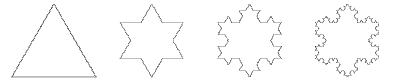
\includegraphics[width=0.5\linewidth]{kochSnowflake.png}
    \caption{First Four Iterations of the Koch Snowflake}
    \label{fig:koch_snowflake}
\end{figure}
\begin{exercise}
Suppose that we create a Koch snowflake with a starting triangle with sides of length 1.
    \begin{enumerate}
        \item At iteration $n$, the perimeter of the Koch Snowflake is given by $L_n = 3\cdot 4^n$.  Prove that the perimeter of the Koch Snowflake in the limit as $n \to \infty$ is infinite.
        \item At iteration $n$, the area of the Koch snowflake is given by
        \begin{align*}
            \frac{2\sqrt3}5 - \frac{3\sqrt3}{20}\cdot \left(\frac49\right)^n.
        \end{align*}
        Prove that as $n \to \infty$, the area is finite, and compute the area.
    \end{enumerate}
\end{exercise}

Fun facts about fractals
\begin{itemize}
    \item Remember the ``old" days when you had to pull out a very large antenna out of TVs (the infamous ``bunny ears")?  Nathan Cohen, a radio astronomer, was living in his apartment and was havin trouble with good reception for his TV set.  He went to a conferences, where Manelbrot showed the audience images of fractals.  He took a wire and bent it in the shape of a Kock Snowflake to the best of his ability and attached it a TV anda  radio.  Immediately, stations and channels were clearer. This was the first discovery that fractal antennas allowed for a broader range of wavelengths with a smaller antenna.  This is also the same reason we do not have to pull antennas out of our phones anymore either.  \textit{Fun fact: Cohen's company contracts for the US military.  Don't research this too much, or you may get a black helicopter flying over your dorm, speaking from experience...}
    \item Fractal research with MRIs increased early detection of breast cancer; additional tumors were discovered in 40\% of patients, changing treatment for 25\% of the patients in the study.
\end{itemize}

\end{document}